\subsection{Имитационная модель. Схема эксперимента}

Для верификации развиваемых в работе подходов можно использовать данные, полученные при захвате в режиме реального времени или же
специально сгенерированные данные с использованием аппаратной или программной платформы. Преимуществом второго подхода
является то, что мы изначально знаем количество источников сигнала и их параметры (частоту, фазу ПСП, количество отраженных лучей).
В данной работе для верификации предложенных подходов будет использоваться второй подход.

В разделе 1 уже рассматривались источники помех в системе с расширенным спектром Navstar GPS:
\begin{itemize}
	\item {данные эфемерид - ошибки в позициях спутников;}
	\item {часы спутника - ошибки в переданных данных о времени;}
	\item {ионосфера - ошибки в коррекции псевдодальностей обусловленных ионосферными эффектами;}
	\item {тропосфера - ошибки в коррекции псевдодальностей обусловленных обусловленных тропосферными эффектами;}
	\item {многолучевость - эффект отраженных сигналов принятых антенной;}
	\item {приемник - ошибки в измерениях обусловленные термальным шумом, точностью ПО и т.д.}
\end{itemize}

Генераторы сигнала можно разделить на программные и аппаратные. Программные генераторы позволяют сгенерировать
ВЧ сигнал с заранее заданными параметрами. В качестве аппаратных платформ для генерации сигнала можно использовать, например,
NI GPS Simulator. Данное решение позволяет сгенерировать практически произвольный сигнал за
счет большого количества настраиваемых параметров. Вместе с тем, аппаратные решения обладают существенным недостатком - высокая цена.

В данной работе будет использован программный подход к генерации сигнала с расширенным спектром. В качестве модели была выбрана модель
сигнала с расширенным спектром СНС Navstar GPS. Существует много программных моделей данного сигнала,
например \cite{hannah_phd, burns_model, corbell_model, crs_model, brown_model}.

\subsection{Схема эксперимента}
Для проверки развиваемых в данной работе подходов построена имитационная модель системы передачи данных с ШПС.
Модель сигнала представлена в выражении \ref{eq:gps_signal}. Так как в работе развивается два подхода для сигнала
с АБГШ и с интерференционной помехой. Имитационная модель должна позволять выбрать необходимое количество источников сигнала.
Для проверки усовершенствованного алгоритма вычисления АКФ для компенсации окрашенной и белой аддитивной шумовой помехи
имитационная модель должна позволять добавлять АБГШ к генерируемому сигналу. 

Функциональная схема системы передачи информации представлена на рисунке \ref{pic:sec4_modeling_general}. Как уже было отмечено, бит данныx ${D_k(t)}$
принят за константу, так при ДФМ переход нарушает гармоническую структуру входного сигнала и детектирование становится невозможным,
она учтена в модели как неизвестная начальная фаза. Несущая сигнала модулируется заданной ПСП с периодом 1023 и длительностью 1 мкс.
Частота сигнала смещена на от центральной частоты для моделирования допплеровского смещения. Рассолгасование и нестабильность
осцилляторов на стороне передатчика учтено в допплеровском смещении. Влияние этого рассогласования крайне невелико в сравнении
со смещением частоты, обусловленным допплеровским смещением в следствии движения передающего и принимающего сегментов.
\noindent
\begin{figure}[ht]
	\center\scalebox{0.65}{\includegraphics[width=1\linewidth]{modeling_general.eps}}
	\caption{Распределение количества источников сигнала}
	\label{pic:sec4_modeling_general}
\end{figure}

К полученному сигналу добавляется ${K}$ (${K}$ может быть равно 0) дополнительных сигналов для создания интерференционной помехи от других источников,
так же добавляется АБГШ. Полученная смесь подавалась на алгоритм детектирования для определения рабочих характеристик развиваемых в работе подходов.

Модель смесиёёё может быть описана как:
\begin{center}
\begin{equation}
	\label{eq:sec4_model}
	x(m) = \sum \limits_{k=1}^{G} \left[ C_k(m)\cos(\omega_{k}m + \phi_k(m)) \right] + n(m)
\end{equation}
\end{center}
где ${C_k(t)}$ - ПСП для ${k}$ - сигнала, ${\omega_{k}}$ - частота несущей ${k}$ - сигнала, ${\phi_k(m)}$ - начальная фаза,
равномерно распределена ${[-\pi, \pi]}$, ${G}$ - количество источников сигнала, ${n(m)}$ - АБГШ.

Количество источников сигнала ${G}$ задается с учетом распределения вероятностей количества источников для конктретной системы
связи с расширенным спектром. Например, для системы Navstar GPS это распределение задается графиком (график приведен из стандарта
Navstar GPS \cite{gpsuserequipment}):
\begin{figure}[ht]
	\center\scalebox{1}{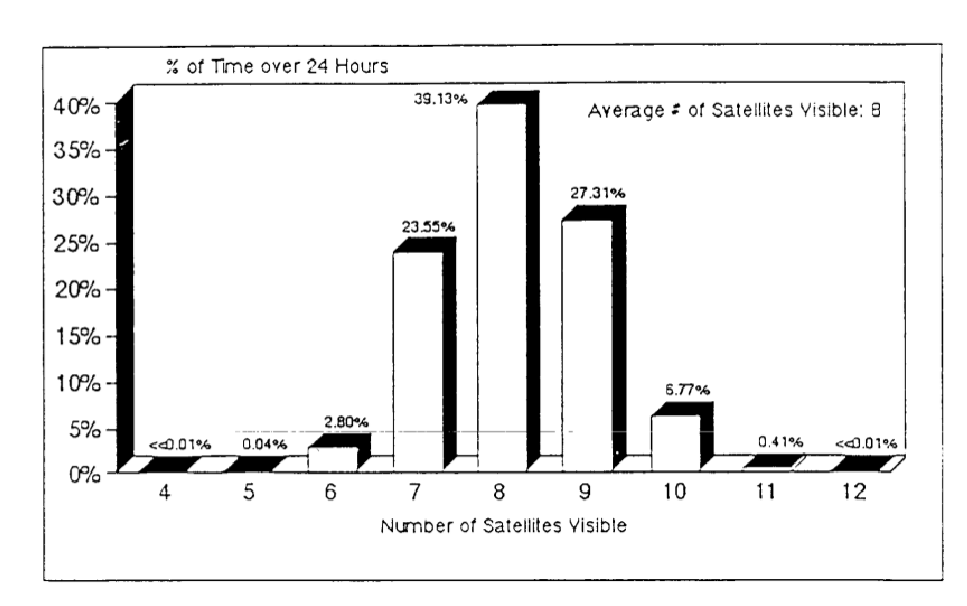
\includegraphics[width=1\linewidth]{gps_sats_num.eps}}
	\caption{Распределение количества источников сигнала}
	\label{pic:sec4_gps_num_of_sats}
\end{figure}

%%%%%%%%%%%%
\subsection{Алгоритм для сравнения по точности}

Для сравнения возьмем программный приемник Navstar GPS рассмотренный в \cite{tsui, akos-book}. 
После стадии детектирования сигнала оценка частоты для заданного источника поступает в модуль уточнения частоты. Уточненная частота и фаза ПСП
поступают в ФАПЧ.  Одним из параметров системы ФАПЧ является шумовая полоса. Этот параметр определяет количество теплового шума попадающего в систему ФАПЧ.
Широкая шумовая полоса позволяет системе ФАПЧ быстро войти в синхронизм, но также ведет к существенному ухудшению характеристик системы ФАПЧ за счет
возрастания уровня теплового шума.  Как уже было рассмотрено ранее область допустимой расстройки частоты определяется как \cite{spilker-book}:
\begin{center}
\begin{eqnarray}
	\label{eq:sec4_pll_omega_m}
	\Delta \omega_m \approx 2 \omega_n (\zeta + 0.6)
\end{eqnarray}
\end{center}
где ${\omega_n}$ - собственная частота системы ФАПЧ, ${\zeta}$ - коэффициент демпфирования (выражение \ref{eq:sec4_pll_omega_m} имеет место,
только при ${\zeta > 0.3}$).

Примем ${\zeta=0.707}$. Данное значение ${\zeta}$ близко к оптимальному \cite{tsui, spilker-book},
тогда ${\Delta \omega_m = 2.614 \omega_n}$. Собственная частота системы ФАПЧ вычисляется по формуле:
\begin{center}
\begin{eqnarray}
	\label{eq:sec4_pll_omega_n}
	\omega_n = \frac{8 \zeta B_L}{4 \zeta^2 + 1}
\end{eqnarray}
\end{center}
где ${B_L}$ - шумовая полоса.

В данном моделировании рассматривается сигнал Navstar GPS с частотой дискретизации ${F_s=16.368}$ МГц, шум задан в полосе от 0 Гц
до половины частоты дискретизации. Допустимая расстройка на входе ФАПЧ должна быть в пределах 16 Гц. 
Для стационарного приемника диапазон смещения частоты обусловленный допплеровским эффектом \cite{tsui} может находится в диапазоне ${\pm 5}$ кГц.

\subsection{Экспериментальная проверка метода детектирования и оценки параметров сигнала при отсутствии интерференции на основе АР-модели}

Данный алгоритм рассмотрен в разделе \ref{l:sec3_lpc_for_1}. Особенностью данного алгоритма является является возможность детектирования сигнала
без перебора по частоте и позиции кода, в том смысле, в котором это понимается в параллельном корреляторе. Оценка частоты производится с
использованием АР-модели.

Таким образом для проверки предложенного алгоритма необходимо в имитационной модели задать один источник сигнала (${G=1}$) и задать уровень АБГШ для
тестирования рабочих характеристик предложенного алгоритма. Моделирование проводилось с аддитивным шумом, заданным в полосе от 0 Гц до
половины частоты дискретизации ${F_s=16.368}$ МГц.

График СКО при оценке частоты в зависимости от ОСШ представлен на рисунке \ref{pic:crlb_vs_1sat_algo}
\begin{figure}[H]
\center\scalebox{1}{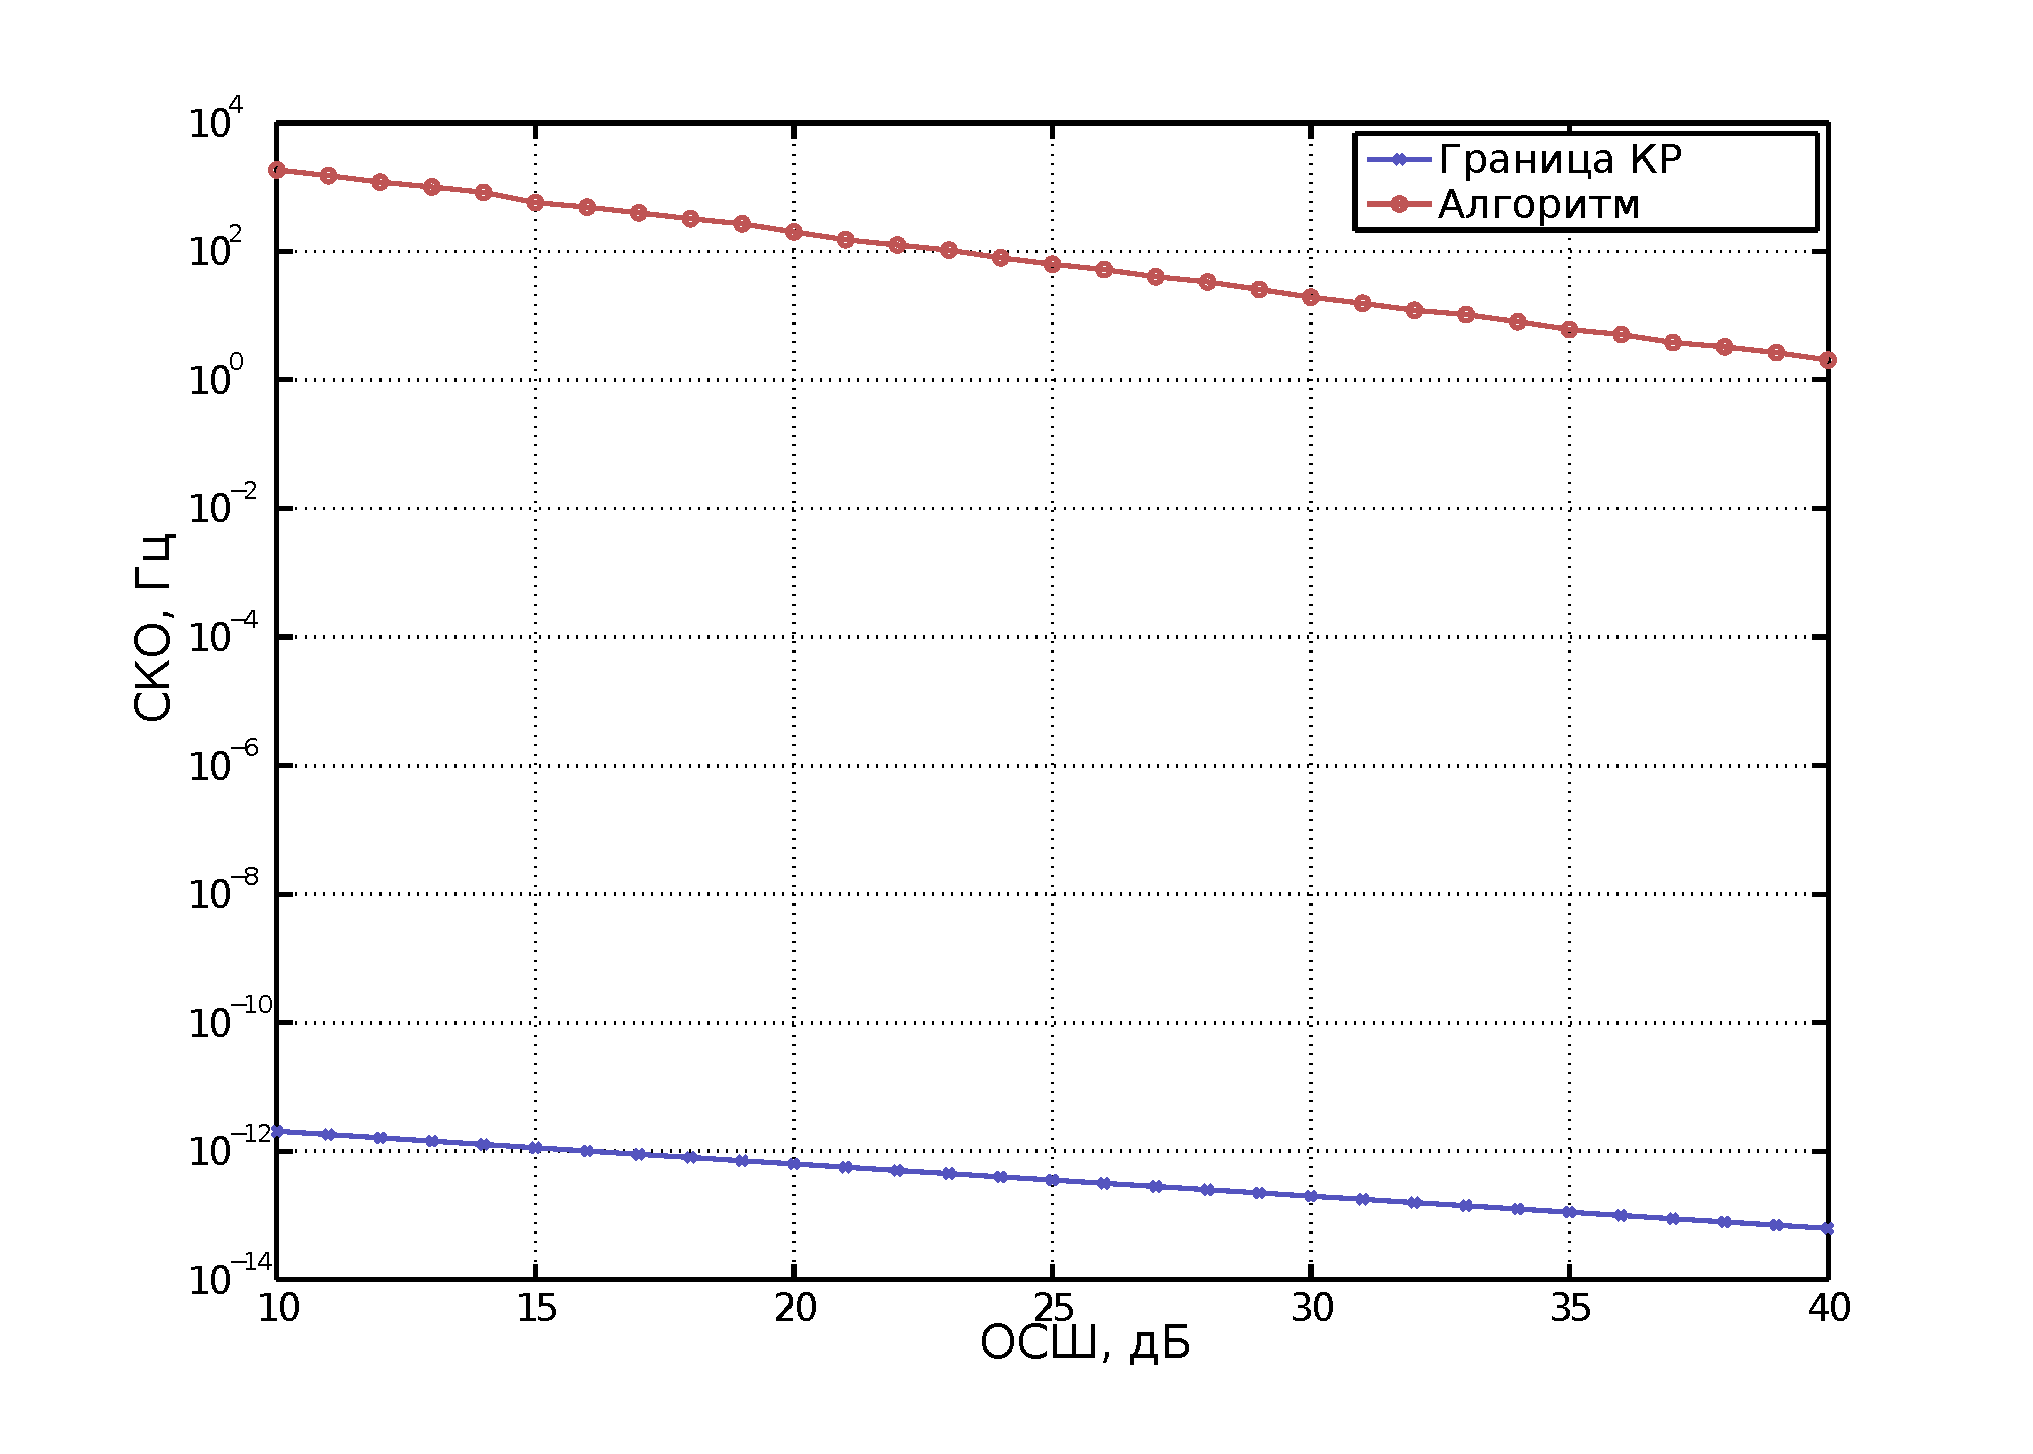
\includegraphics[width=1\linewidth]{crlb_vs_1sat_algo.eps}}
	\caption{СКО ошибка оценки частоты и граница Крамера-Рао в задаче оценки частоты гармонического сигнала}
	\label{pic:crlb_vs_1sat_algo}
\end{figure}

График вероятности оценки частоты в допустимом диапазоне входной расстройки представлен на рисунке
\ref{pic:lpc_for_1_probability}. 
\begin{figure}[H]
\center\scalebox{1}{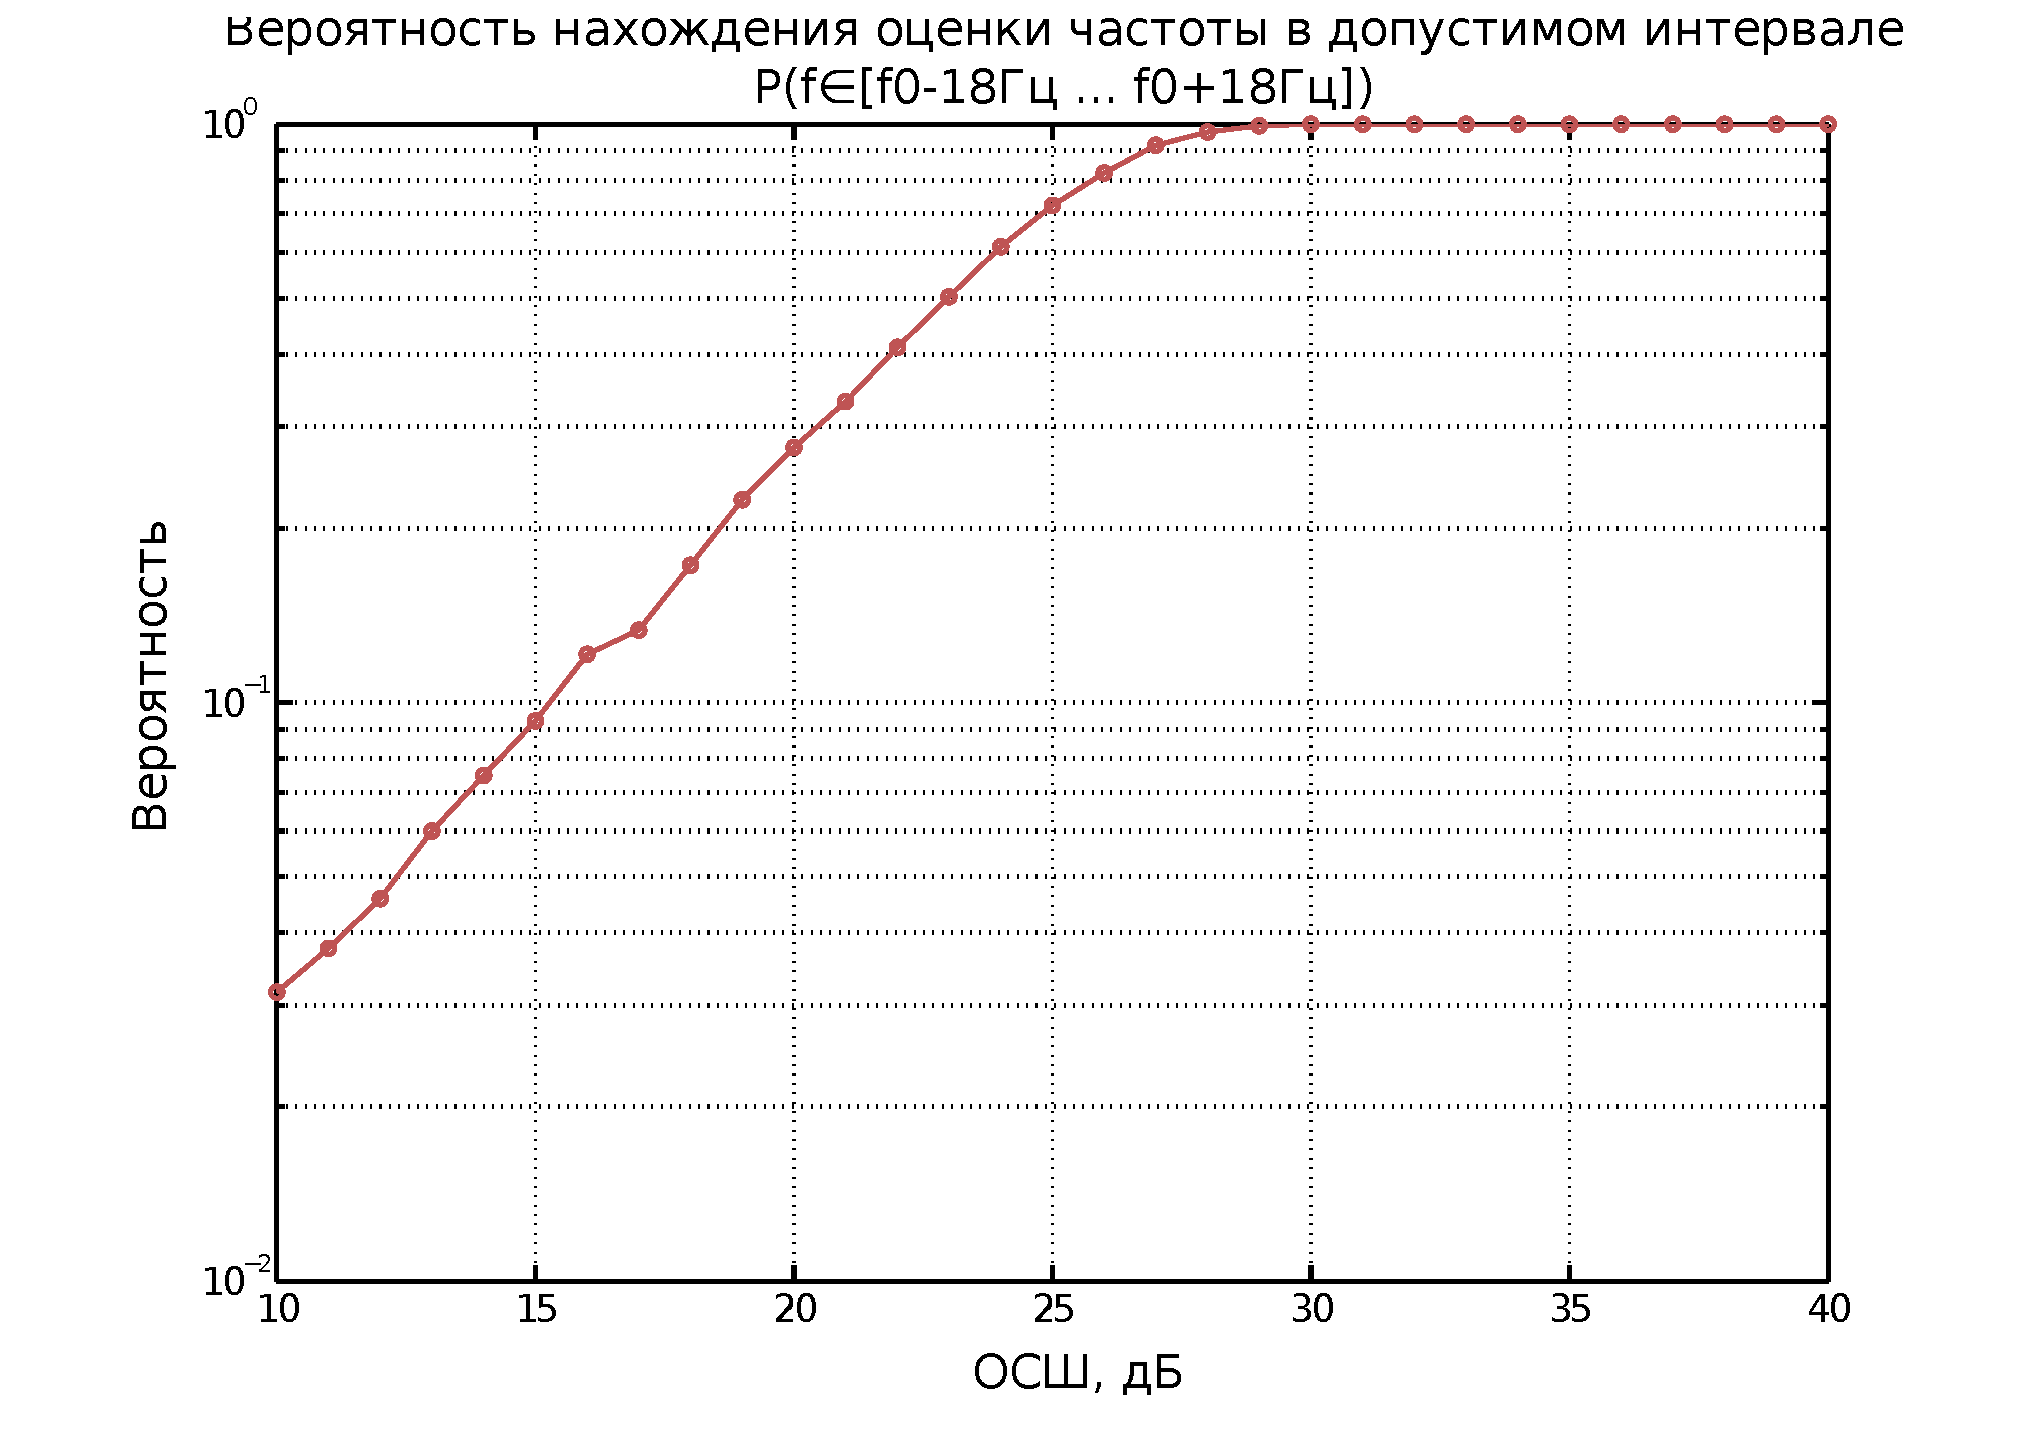
\includegraphics[width=1\linewidth]{lpc_for_1_probability.eps}}
	\caption{Вероятность оценки частоты удовлетворяющей допустимой входной расстройке}
	\label{pic:lpc_for_1_probability}
\end{figure}

\subsection{Экспериментальная проверка метода детектирования и оценки параметров сигнала на основе АР-модели с использованием уточненной оценки АКФ
	и алгоритма Delay and Multiply Approach}

Данный алгоритм рассмотрен в разделе \ref{l:ssec3_dma_lpc_algo}. Данный алгоритм позволяет детектировать и оценивать параметры сигнала с расширенным спектром
на фоне АБГШ и интерференционной помехи. Таким образом для оценки данного алгоритма необходимо добавить ко входной смеси АБГШ и интерференционную помеху
для тестирования рабочих характеристик предлагаемого подхода.

График вероятности оценки частоты в допустимом даипазоне входной расстройки представлен на рисунке
\ref{pic:ar_dma_probability}. Моделирование проводилось с аддитивным шумом, заданным в полосе от 0 Гц до
половины частоты дискретизации ${F_s=16.368}$ МГц для одного, двух и трех шагов уточнения АКФ. В данном случае ${G=4}$ - 
один источник сигнала в качестве основного для поиска и оценки частоты и 3 дополнительных для создания интерференционной помехи.
\begin{figure}[H]
\center\scalebox{1}{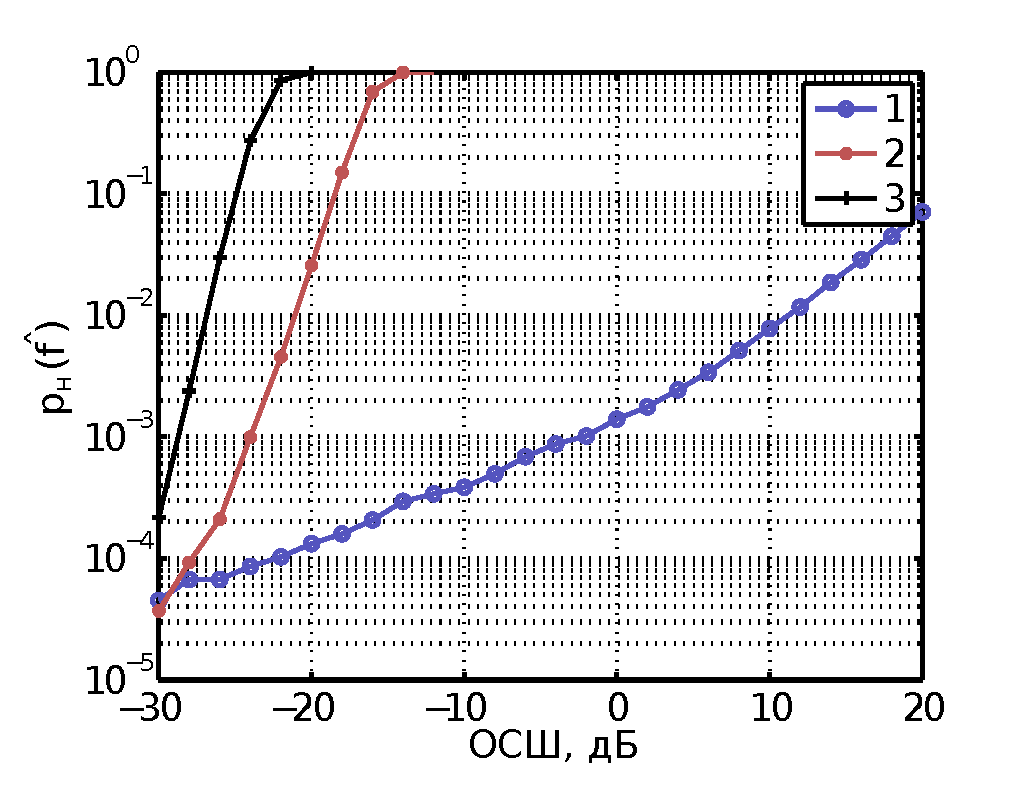
\includegraphics[width=1\linewidth]{ar_dma_probability.eps}}
	\caption{Вероятность оценки частоты удовлетворяющей допустимой расстройке}
	\label{pic:ar_dma_probability}
\end{figure}

%Предлагаемый подход существенно выигрывает по вычислительным затратам в сравнении с параллельным коррелятором при
%меньших вычислительных затратах.

Так же интересным является сравнение качества оценки частоты. График СКО ошибки при оценке частоты в зависимости
от ОСШ представлен на рисунке \ref{pic:crlb_vs_snr}. Для сравнения так же взята граница Крамера-Рао (КР).
\begin{figure}[H]
\center\scalebox{1}{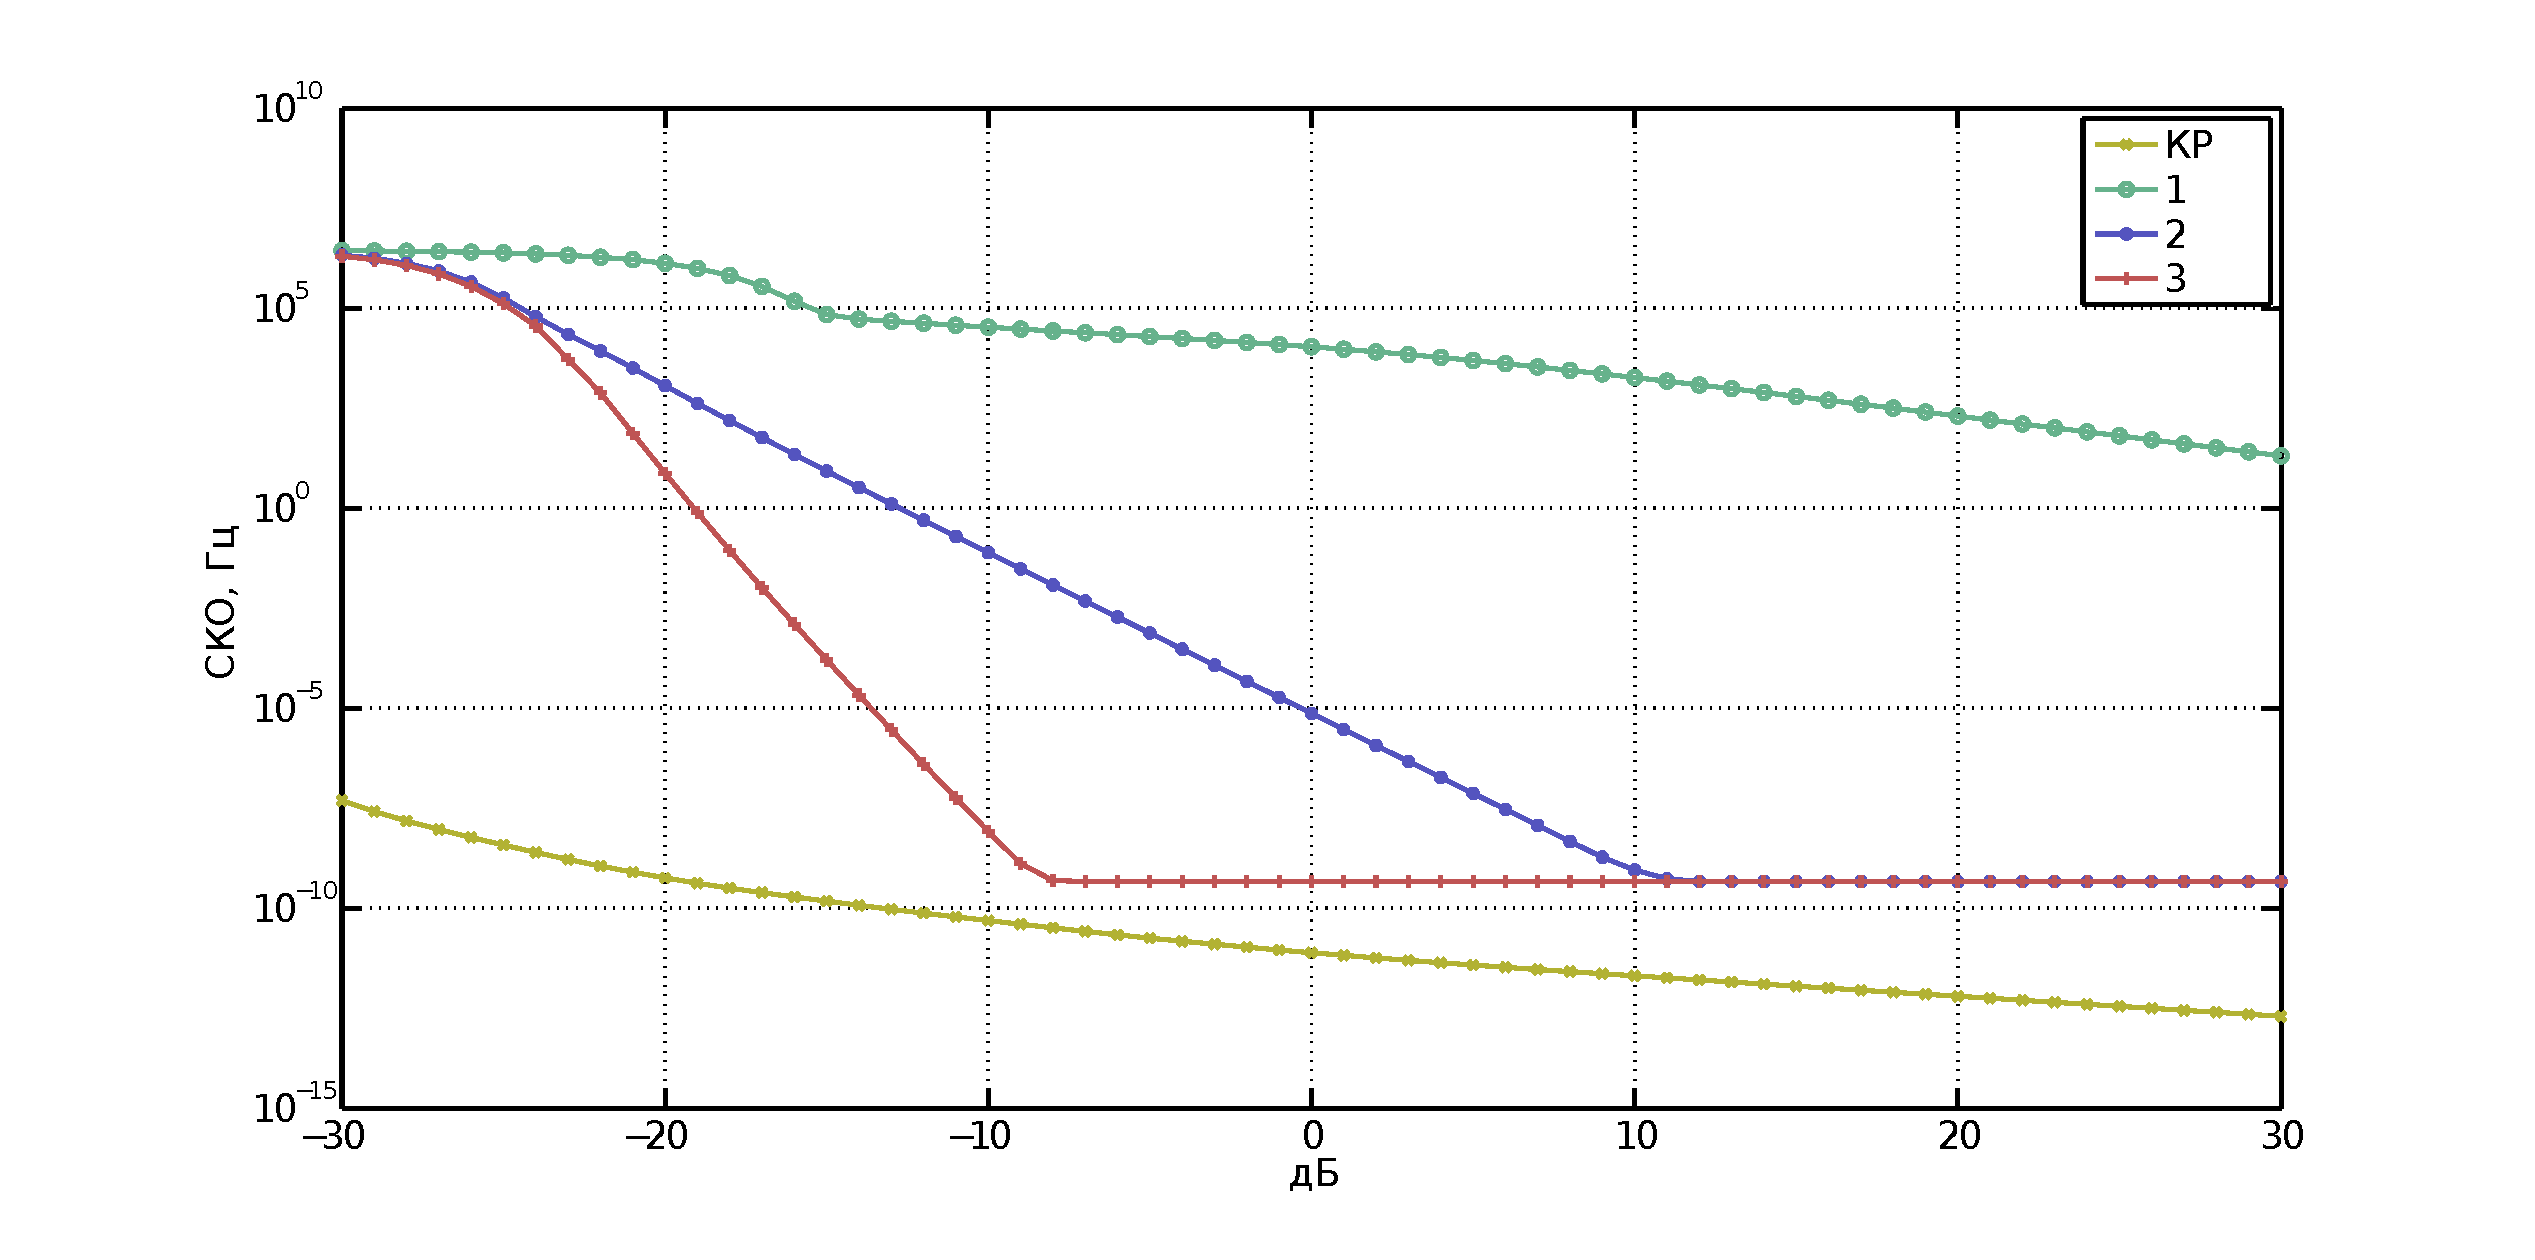
\includegraphics[width=1\linewidth]{crlb_vs_snr.eps}}
	\caption{СКО ошибка оценки частоты и граница Крамера-Рао в задаче оценки частоты гармонического сигнала}
	\label{pic:crlb_vs_snr}
\end{figure}

\newpage
